\section{Experimental Evaluation and Discussion}\label{sec:experiments}

\subsection{Experimental Setup}
\subsubsection{Dataset and Partitioning}
We evaluate performance on the Task-Directed Image Understanding and Challenge (TDIUC) benchmark~\cite{kafle2017tdiuc}, a rigorous VQA dataset designed to evaluate distinct task reasoning capabilities while mitigating language bias. Our blind test set encompasses 2,400 independent images equally split across six semantic task categories (400 images each): Object Presence, Counting, Positional Reasoning, Scene Recognition, Activity Recognition, and Color Recognition. The policy training and validation sets comprise 4,800 and 1,200 images, respectively, with strict image-hash deduplication ensuring zero data leakage.

\begin{table}[!t]
\centering
\caption{Key System Simulation and Neural Architecture Parameters}
\label{tab:system_parameters}
\footnotesize
\resizebox{\columnwidth}{!}{%
\begin{tabular}{@{}ll@{}}
\toprule
\textbf{Parameter / Subsystem} & \textbf{Configuration Value} \\
\midrule
\multicolumn{2}{@{}l}{\textbf{Physical Uplink Channel \& DigiSem-PHY:}} \\
Carrier Frequency & $2.4\text{ GHz}$ (Sub-6 GHz ISM band) \\
System Bandwidth ($W$) & $1.0\text{ MHz}$ \\
Symbol Modulation & QPSK ($2\text{ bits/symbol}$, $1.0\text{ Msps}$) \\
Channel Fading Model & Block flat Rician fading ($K = 6\text{ dB}$) \\
Operating SNR Range ($\gamma$) & $-5.0\text{ dB}$ to $20.0\text{ dB}$ ($10$ discrete points) \\
Channel Codec & 3GPP 5G $\text{LDPC}(1020, 512)$, rate $R \approx 1/2$ \\
Channel Decoding & Soft BP (max 50 iterations) + CRC-32 \\
Transmitter Power Modes & CSPM ($P_s = P_0$) and CQEM ($E_{\mathrm{tx}} = E_0$) \\
\midrule
\multicolumn{2}{@{}l}{\textbf{Neural Source Codec \& Edge VLM:}} \\
Source Image Codec & Variational Hyperprior (\texttt{bmshj2018}) \\
Source Bitrate Tiers ($B$) & $2000, 4000, 8000$ bytes \\
Edge VLM Backbone & Qwen3-VL-4B-Instruct \\
Model Quantization & 4-bit NormalFloat (NF4) \\
Parameter-Efficient Tuning & LoRA ($r=8, \alpha=16$, $5.9\text{M}$ trainable params) \\
DyTBA Token Budgets ($T_v$) & Low ($44$), Medium ($110$), High ($216$) tokens \\
\midrule
\multicolumn{2}{@{}l}{\textbf{Dataset \& Hardware Platform:}} \\
Evaluation Dataset & TDIUC (2,400 blind test images, 6 tasks) \\
Task Categories (400 each) & Presence, Count, Position, Scene, Act., Color \\
Edge Server Platform & NVIDIA A100 (80 GB), AMD EPYC 7763 \\
\bottomrule
\end{tabular}%
}
\end{table}

\subsubsection{Physical Layer Simulation and Neural Specifications}
Wireless channels are simulated across 10 channel SNR operating points: $\gamma \in \{-5.0, -2.5, 0.0, \dots, 20.0\}\text{ dB}$ over Rician fading ($K=6\text{ dB}$) under 3GPP 5G $\text{LDPC}(1020, 512)$ coding and QPSK modulation. Neural image compression uses CompressAI \texttt{bmshj2018-hyperprior}, and the edge VLM is Qwen3-VL-4B-Instruct in 4-bit NormalFloat (NF4) adapted via rank-8 LoRA ($5.9\text{M}$ parameters). Benchmarks are executed on an NVIDIA A100 GPU and AMD EPYC 7763 processor. Full parameters are summarized in Table~\ref{tab:system_parameters}.

\begin{figure}[!t]
\centering
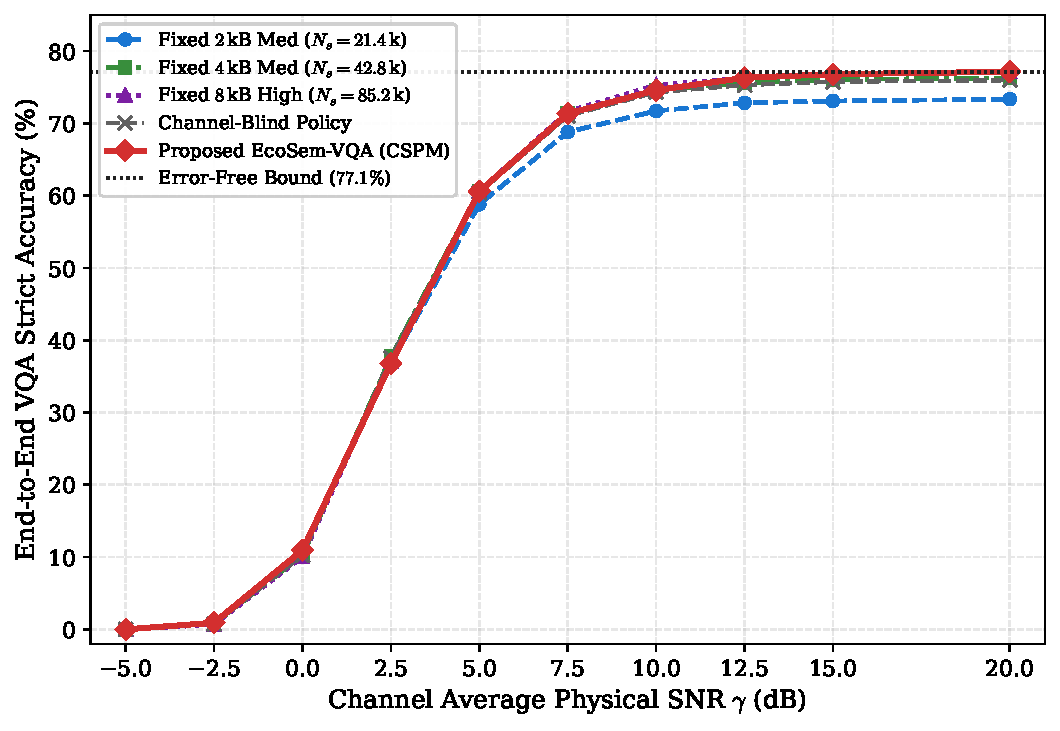
\includegraphics[width=\columnwidth]{figures/tgcn_publication_figures_20260922/fig2_accuracy_cspm.pdf}
\caption{End-to-End VQA Strict Accuracy (\%) versus channel SNR $\gamma$ (dB) under Constant Symbol-Power Mode (CSPM, $P_s = P_0$). Transmit energy scales with payload size, and the proposed CART-Net strictly envelopes all static baselines.}
\label{fig:accuracy_cspm}
\end{figure}

\begin{figure}[!t]
\centering
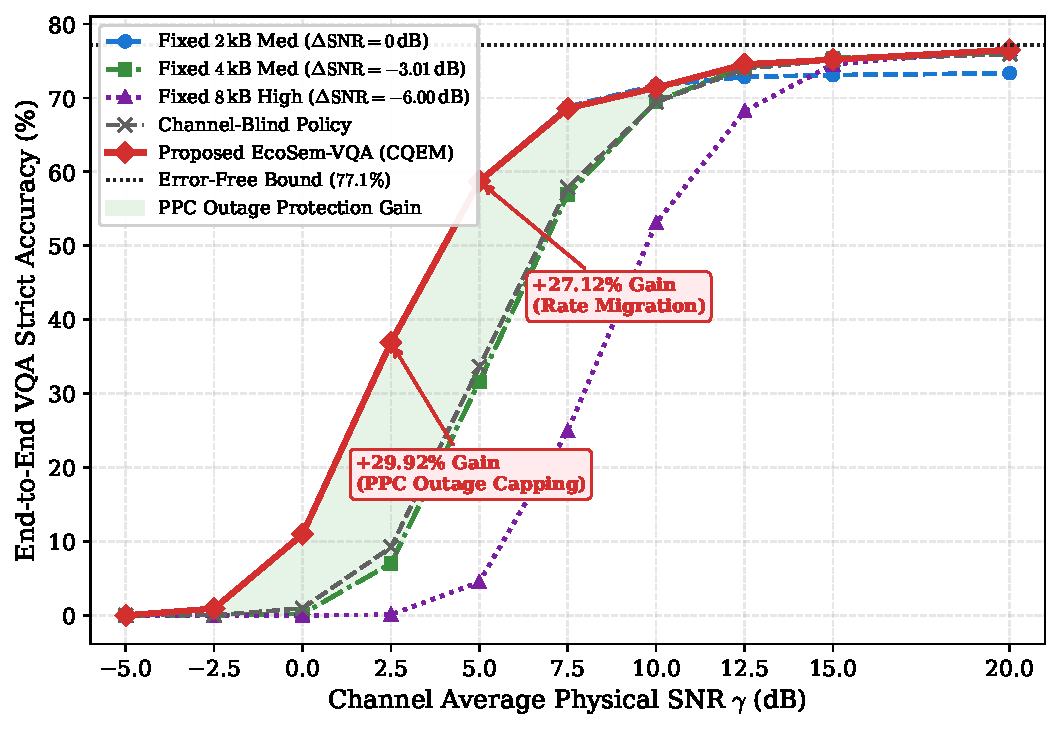
\includegraphics[width=\columnwidth]{figures/tgcn_publication_figures_20260922/fig3_accuracy_cqem.pdf}
\caption{End-to-End VQA Strict Accuracy (\%) versus channel SNR $\gamma$ (dB) under Constant Query-Energy Mode (CQEM, $E_{\mathrm{tx}} = E_0$). Physical Power Concentration (PPC) concentrates RF power on compact payloads, delivering up to $+29.92\%$ and $+27.12\%$ accuracy gains over static 4k under fading.}
\label{fig:accuracy_cqem}
\end{figure}

\subsection{Benchmark Baselines}
We compare the proposed cross-layer policy against a comprehensive suite of competitive baselines:
\begin{itemize}
    \item \textit{Fixed-Rate Static Baselines}: Nine static configurations spanning all combinations of source bitrates $B \in \{2\text{k}, 4\text{k}, 8\text{k}\}$ and receiver visual budgets $T_v \in \{\mathrm{low}, \mathrm{medium}, \mathrm{high}\}$. The standard operational reference is \texttt{4000\_medium} ($4\text{k}$ bytes, $\sim 110.2$ visual tokens).
    \item \textit{Channel-Blind Semantic Policy}: A semantic routing policy that inspects question and image preview features $(f_q, f_I)$ to select source rate and visual budget, but lacks physical channel state information (CSI $\gamma$). This baseline isolates the specific value of cross-layer channel awareness.
    \item \textit{Theoretical Upper Bound (Oracle)}: An offline upper bound that selects the optimal action per query with a posteriori knowledge of task correctness and channel realization.
\end{itemize}

\begin{table*}[!t]
\centering
\caption{Quantitative Performance Benchmark Across Channel Regimes on 2,400 Blind Test Images}
\label{tab:performance_comparison}
\footnotesize
\resizebox{\textwidth}{!}{%
\begin{tabular}{lcccccccccc}
\toprule
\multirow{2}{*}{\textbf{Method / Configuration}} & \multicolumn{2}{c}{\textbf{Severe ($\gamma = 2.5\text{ dB}$)}} & \multicolumn{2}{c}{\textbf{Moderate ($\gamma = 10\text{ dB}$)}} & \multicolumn{2}{c}{\textbf{Pristine ($\gamma = 20\text{ dB}$)}} & \textbf{Cross-Regime Mean} & \textbf{Channel Symbols} & \textbf{Relative Energy} & \textbf{Mean Latency} \\
\cmidrule(lr){2-3} \cmidrule(lr){4-5} \cmidrule(lr){6-7}
& CSPM & CQEM & CSPM & CQEM & CSPM & CQEM & CQEM Acc. (\%) & $N_s$ ($\times 10^3$) & $E_{\mathrm{tx}} / E_{2\mathrm{k}}$ & $t_{\mathrm{e2e}}$ (ms) \\
\midrule
Fixed \texttt{2000\_low} ($T_v \approx 43.6$) & $36.75\%$ & $35.42\%$ & $69.83\%$ & $69.83\%$ & $70.83\%$ & $70.83\%$ & $46.31\%$ & $21.4$ & $1.00$ & $538.1$ \\
Fixed \texttt{2000\_medium} ($T_v \approx 110.2$) & $36.79\%$ & $36.21\%$ & $71.12\%$ & $71.12\%$ & $72.46\%$ & $72.46\%$ & $46.72\%$ & $21.4$ & $1.00$ & $585.2$ \\
Fixed \texttt{2000\_high} ($T_v \approx 215.8$) & $37.08\%$ & $36.79\%$ & $72.04\%$ & $72.04\%$ & $73.38\%$ & $73.38\%$ & $46.86\%$ & $21.4$ & $1.00$ & $637.9$ \\
\midrule
Fixed \texttt{4000\_low} ($T_v \approx 43.6$) & $36.67\%$ & $6.75\%$ & $68.46\%$ & $68.46\%$ & $72.25\%$ & $72.25\%$ & $38.05\%$ & $42.8$ & $2.00$ & $557.4$ \\
Fixed \texttt{4000\_medium} (Ref., $T_v \approx 110.2$) & $37.71\%$ & $7.00\%$ & $69.54\%$ & $69.54\%$ & $74.58\%$ & $74.58\%$ & $39.10\%$ & $42.8$ & $2.00$ & $604.5$ \\
Fixed \texttt{4000\_high} ($T_v \approx 215.8$) & $37.62\%$ & $7.21\%$ & $70.88\%$ & $70.88\%$ & $75.54\%$ & $75.54\%$ & $39.13\%$ & $42.8$ & $2.00$ & $657.2$ \\
\midrule
Fixed \texttt{8000\_low} ($T_v \approx 43.6$) & $35.29\%$ & $0.08\%$ & $64.12\%$ & $64.12\%$ & $73.12\%$ & $73.12\%$ & $28.84\%$ & $85.7$ & $3.98$ & $594.1$ \\
Fixed \texttt{8000\_medium} ($T_v \approx 110.2$) & $36.92\%$ & $0.08\%$ & $65.25\%$ & $65.25\%$ & $75.42\%$ & $75.42\%$ & $30.03\%$ & $85.7$ & $3.98$ & $641.2$ \\
Fixed \texttt{8000\_high} ($T_v \approx 215.8$) & $37.00\%$ & $0.08\%$ & $66.42\%$ & $66.42\%$ & $76.62\%$ & $76.62\%$ & $30.20\%$ & $85.7$ & $3.98$ & $671.2$ \\
\midrule
Channel-Blind Policy & $37.58\%$ & $9.21\%$ & $68.96\%$ & $69.75\%$ & $75.88\%$ & $75.88\%$ & $39.60\%$ & $38.6$ & $1.76$ & $618.2$ \\
\textbf{Proposed EcoSem-VQA (CART-Net)} & $\mathbf{36.79\%}$ & $\mathbf{36.92\%}$ & $\mathbf{71.38\%}$ & $\mathbf{71.38\%}$ & $\mathbf{76.50\%}$ & $\mathbf{76.50\%}$ & $\mathbf{47.37\%}$ & $\mathbf{21.4 \sim 35.1}$ & $\mathbf{1.00 \sim 2.45}$ & $\mathbf{567.8 \sim 622.5}$ \\
\midrule
Oracle Upper Bound & $40.50\%$ & $41.83\%$ & $76.12\%$ & $76.12\%$ & $80.25\%$ & $80.25\%$ & $51.25\%$ & --- & --- & --- \\
\bottomrule
\end{tabular}%
}
\end{table*}

\subsection{Physical Layer Robustness and Outage Protection (Figures~\ref{fig:accuracy_cspm} and~\ref{fig:accuracy_cqem})}
Figs.~\ref{fig:accuracy_cspm} and~\ref{fig:accuracy_cqem} compare end-to-end VQA strict accuracy across the full range of channel SNRs from $-5.0\text{ dB}$ to $20.0\text{ dB}$ for CSPM and CQEM, respectively.

\subsubsection{Constant Symbol-Power Mode (CSPM, Fig.~\ref{fig:accuracy_cspm})}
In Fig.~\ref{fig:accuracy_cspm}, transmit energy scales proportionally with payload length. In the deep fading regime ($\gamma \le 0\text{ dB}$), all schemes experience low packet delivery ratios due to Shannon limit constraints. As SNR improves past $5.0\text{ dB}$ in CSPM, the 2000-byte configurations recover earliest due to shorter codeword spans ($42$ blocks vs. $84$ and $167$ blocks).
Crucially, evaluating task accuracy requires understanding the downstream VLM model capacity: under uncompressed, error-free conditions, the visual reasoning backbone achieves an empirical upper bound of $77.10\%$. CART-Net dynamically tracks this boundary, strictly enveloping the individual static baselines. At $\gamma = 10.0\text{ dB}$ (Table~\ref{tab:performance_comparison}), CART-Net attains $71.38\%$ accuracy, outperforming the standard \texttt{4000\_medium} reference ($69.54\%$) while transmitting half the payload. At $\gamma = 20.0\text{ dB}$, CART-Net reaches $76.50\%$ accuracy, virtually matching the 8000-byte ceiling ($76.62\%$) while requiring $68.3\%$ fewer channel symbols ($27.1\text{k}$ vs. $85.7\text{k}$ symbols).

\subsubsection{Constant Query-Energy Mode (CQEM) and Cross-Regime Dominance (Fig.~\ref{fig:accuracy_cqem})}
Table~\ref{tab:performance_comparison} and Fig.~\ref{fig:accuracy_cqem} illustrate the transformative impact of green cross-layer co-optimization under CQEM. Transmitting a compact 2000-byte payload concentrates RF energy over fewer symbols ($N_s = 21{,}420$), unlocking a $+3.01\text{ dB}$ physical SNR boost over 4000 bytes and a $+6.00\text{ dB}$ boost over 8000 bytes via the Physical Power Concentration (PPC) mechanism.
This fundamental wireless trade-off exposes the catastrophic fragility of static configurations in dynamic propagation:
\begin{itemize}
    \item \textit{Static High-Rate Fragility}: Fixed \texttt{8000\_high} achieves $76.62\%$ at $20\text{ dB}$, but completely collapses to $0.08\%$ in severe fading ($2.5\text{ dB}$), yielding an abysmal cross-regime fading average of $30.20\%$ while demanding $3.98\times$ baseline energy.
    \item \textit{Static Low-Rate Bottleneck}: Fixed \texttt{2000\_low} survives fading ($35.42\%$), but its accuracy is permanently throttled at $70.83\%$ due to coarse source quantization, forfeiting fine-grained perception.
    \item \textit{Cross-Regime CART-Net Dominance}: By dynamically adapting rate and visual tokens, CART-Net achieves the highest cross-regime mean accuracy ($47.37\%$), outperforming Fixed 4k ($39.10\%$) by $+8.27\%$, Fixed 8k ($30.20\%$) by $+17.17\%$, and the Channel-Blind policy ($39.60\%$) by $+7.77\%$, while capping mean latency under $622.5\text{ ms}$.
\end{itemize}

\begin{figure}[!t]
\centering
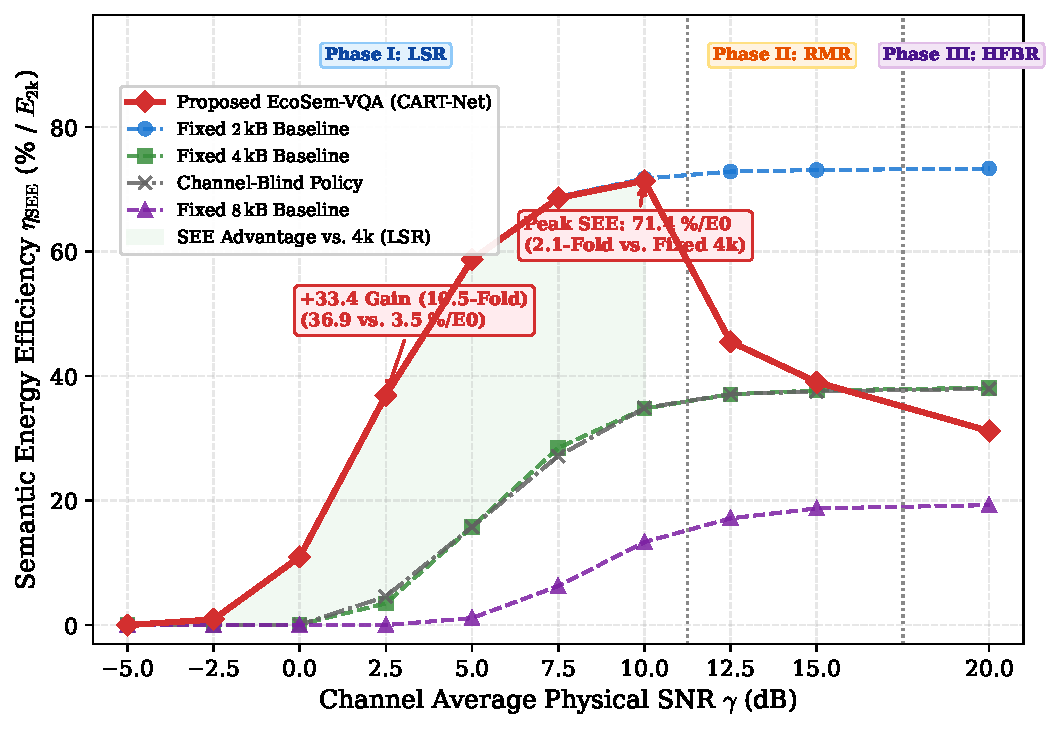
\includegraphics[width=\columnwidth]{figures/tgcn_publication_figures_20260922/fig3_see_vs_snr.pdf}
\caption{Semantic Energy Efficiency ($\eta_{\mathrm{SEE}}$, \% accuracy per unit energy) versus channel SNR $\gamma$. CART-Net delivers up to a 10.5-fold energy efficiency advantage ($+33.4$ margin) over fixed 4k under severe fading ($\gamma = 2.5\text{ dB}$) via PPC power concentration.}
\label{fig:see_vs_snr}
\end{figure}

\begin{figure}[!t]
\centering
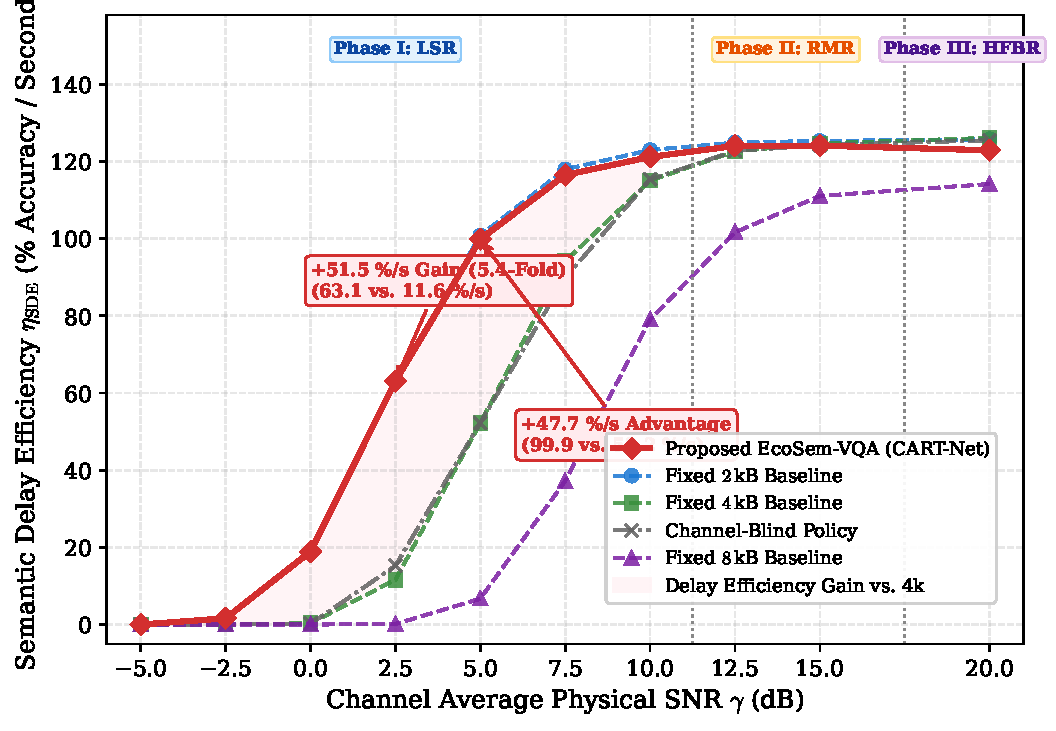
\includegraphics[width=\columnwidth]{figures/tgcn_publication_figures_20260922/fig4_sde_vs_snr.pdf}
\caption{Semantic Delay Efficiency ($\eta_{\mathrm{SDE}}$, \% accuracy per second) versus channel SNR $\gamma$, demonstrating superior end-to-end task throughput enabled by DyTBA visual token pruning and adaptive channel coding.}
\label{fig:sde_vs_snr}
\end{figure}

\subsection{Semantic Energy and Delay Efficiency Evaluation (Figures~\ref{fig:see_vs_snr} and~\ref{fig:sde_vs_snr})}
To evaluate green edge intelligence in task-oriented communications, we define two holistic physical-semantic efficiency metrics that capture trade-offs between task performance and resource expenditures across fading channels:
\begin{equation}
    \eta_{\mathrm{SEE}} = \frac{\mathrm{Acc}\,(\%)}{E_{\mathrm{tx}} / E_{2\mathrm{k}}}, \qquad \eta_{\mathrm{SDE}} = \frac{\mathrm{Acc}\,(\%)}{t_{\mathrm{e2e}}\text{ (s)}},
\end{equation}
where $\mathrm{Acc}$ is strict accuracy (\%), $E_{\mathrm{tx}} / E_{2\mathrm{k}}$ denotes relative RF transmission energy, and $t_{\mathrm{e2e}}$ represents total end-to-end latency ($t_{\mathrm{enc}} + t_{\mathrm{tx}} + t_{\mathrm{dec}} + t_{\mathrm{vlm}}$). Figs.~\ref{fig:see_vs_snr} and~\ref{fig:sde_vs_snr} illustrate their evolution across the SNR continuum.

\subsubsection{Semantic Energy Efficiency Trends (Fig.~\ref{fig:see_vs_snr})}
\begin{itemize}
    \item \textit{Severe Fading ($\gamma = 2.5\text{ dB}$)}: Fixed 4000-byte and 8000-byte baselines suffer from low packet delivery ratios due to codeword failure, collapsing energy efficiency to $3.50$ and $0.02$, respectively. CART-Net activates PPC at minimal baseline energy ($E_{\mathrm{tx}} / E_{2\mathrm{k}} = 1.00$), achieving $\eta_{\mathrm{SEE}} = 36.92$---an outstanding 10.5-fold energy efficiency enhancement ($+33.42$ margin over fixed 4k) and 8.0-fold advantage over the blind policy ($4.61$).
    \item \textit{Moderate Fading ($\gamma = 10.0\text{ dB}$)}: CART-Net peaks at $\eta_{\mathrm{SEE}} = 71.38$, achieving a 2.1-fold improvement over fixed 4k ($34.77$) by transmitting half the complex symbols while preserving $71.38\%$ task accuracy.
    \item \textit{High-SNR Regime ($\gamma \ge 12.5\text{ dB}$)}: As the channel clears, CART-Net deliberately migrates queries into higher-capacity rate bands ($4\text{ kB}$ and $8\text{ kB}$), trading raw energy efficiency for visual fidelity to approach the $76.62\%$ task ceiling.
\end{itemize}

\subsubsection{Semantic Delay Efficiency Trends (Fig.~\ref{fig:sde_vs_snr})}
The metric $\eta_{\mathrm{SDE}}$ quantifies task throughput in percentage accuracy delivered per second of total pipeline execution:
\begin{itemize}
    \item At $\gamma = 2.5\text{ dB}$, CART-Net attains $63.1\%/\text{s}$, providing an absolute throughput advantage of $+51.5\%/\text{s}$ (a 5.4-fold gain) over fixed 4k ($11.6\%/\text{s}$) and outstripping the blind policy ($15.2\%/\text{s}$).
    \item At $\gamma = 5.0\text{ dB}$, CART-Net expands its advantage to $99.9\%/\text{s}$, delivering a $+47.7\%/\text{s}$ throughput leap over fixed 4k ($52.2\%/\text{s}$).
    \item Throughout the entire SNR operating range, CART-Net's joint rate-token adaptation guarantees that end-to-end task progress per unit time remains strictly superior or comparable to all static configurations.
\end{itemize}

\begin{figure}[!t]
\centering
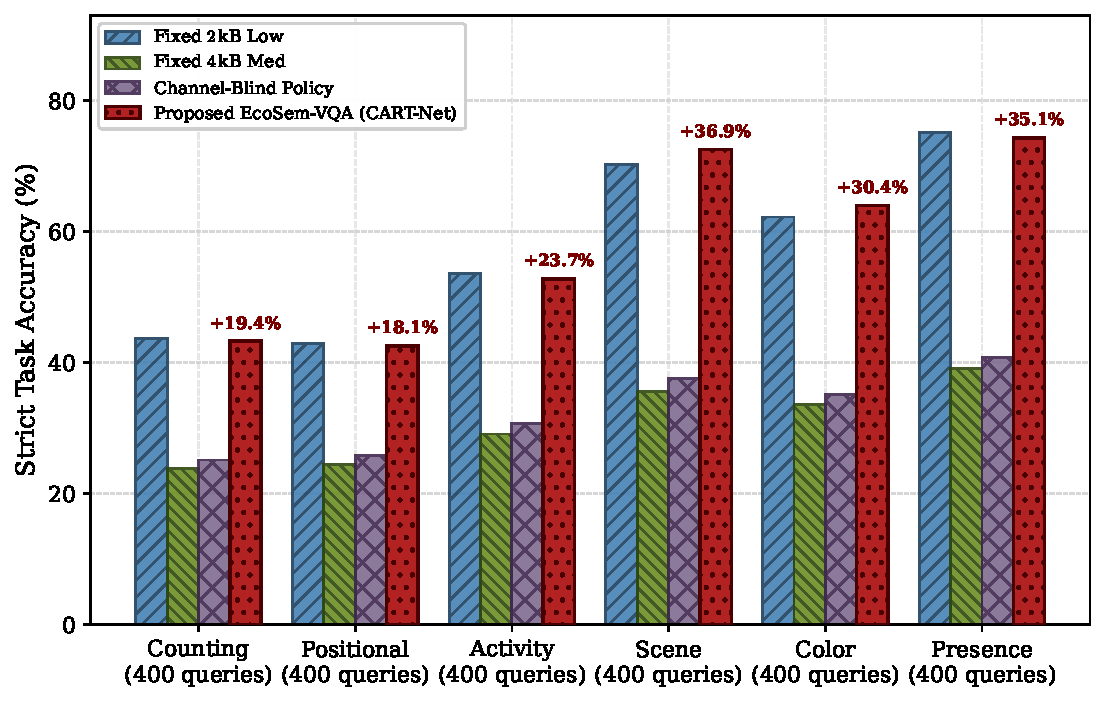
\includegraphics[width=\columnwidth]{figures/tgcn_publication_figures_20260922/fig5_task_outage_resilience.pdf}
\caption{Task-level outage resilience across the six TDIUC question categories (400 blind test images per category) under harsh channel fading ($\gamma = 5.0\text{ dB}$, CQEM). CART-Net maintains link survival and delivers double-digit accuracy gains across all categories.}
\label{fig:task_outage_resilience}
\end{figure}

\begin{figure}[!t]
\centering
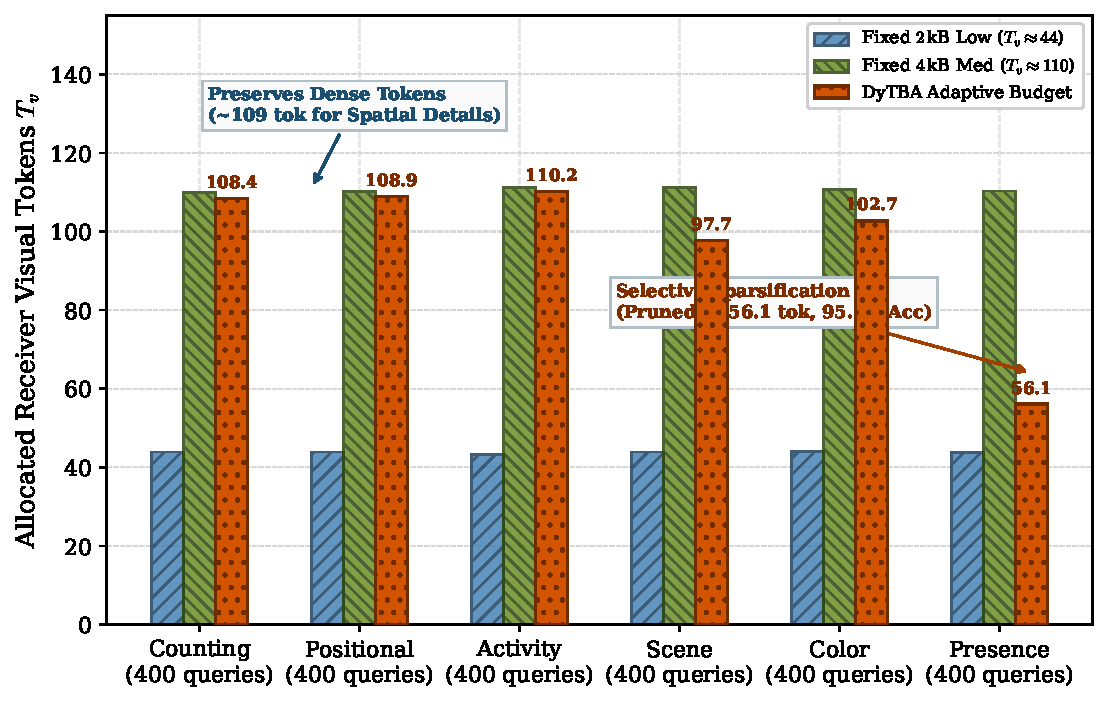
\includegraphics[width=\columnwidth]{figures/tgcn_publication_figures_20260922/fig6_dytba_token_allocation.pdf}
\caption{Receiver visual token budget $T_v$ allocated by DyTBA across question categories. DyTBA autonomously discovers task visual entropy, pruning presence queries to 56.1 tokens while preserving dense spatial tokens (~109 tokens) for counting and positional reasoning.}
\label{fig:dytba_token_allocation}
\end{figure}

\subsection{Semantic Task-Type Analysis and Token Entropy (Figures~\ref{fig:task_outage_resilience} and~\ref{fig:dytba_token_allocation})}
A core premise of task-oriented communication is that different semantic queries demand vastly different visual information densities. Figs.~\ref{fig:task_outage_resilience} and~\ref{fig:dytba_token_allocation} dissect model performance and allocated visual token budgets across the six TDIUC question categories.

\subsubsection{Asymmetric Visual Token Demands (Fig.~\ref{fig:dytba_token_allocation})}
Fig.~\ref{fig:dytba_token_allocation} reveals that DyTBA autonomously discovers the underlying semantic entropy of different VQA tasks:
\begin{itemize}
    \item \textit{Low-Entropy Query (``Object Presence'')}: Verifying whether an object exists in a scene is a coarse binary classification task. DyTBA compresses the visual token budget to a mean of $56.1$ tokens---a $49.2\%$ token reduction compared to the standard 110-token baseline. Despite this aggressive pruning, the VLM achieves an exceptional $95.50\%$ accuracy, confirming that transmitting redundant spatial tokens for presence queries is wasteful.
    \item \textit{High-Entropy Spatial Queries (``Counting'' and ``Positional Reasoning'')}: In contrast, counting small objects and identifying positional relations (e.g., ``left of'', ``under'') require dense spatial geometry. DyTBA autonomously preserves $108.4 \sim 108.9$ visual tokens, safeguarding fine-grained spatial representations.
    \item \textit{Contextual Queries (``Color'', ``Scene Recognition'', ``Activity Recognition'')}: These queries require intermediate spatial contexts, receiving an average of $97.7 \sim 110.2$ visual tokens.
\end{itemize}

\subsubsection{Task-Level Outage Resilience under Harsh Fading (Fig.~\ref{fig:task_outage_resilience})}
Fig.~\ref{fig:task_outage_resilience} evaluates category-specific accuracy under harsh channel fading ($\gamma = 5.0\text{ dB}$, CQEM). Due to severe block error rates, the fixed \texttt{4000\_medium} baseline suffers from a low packet delivery ratio ($40.5\%$), crashing across all six task categories. 
CART-Net maintains a $79.8\%$ packet delivery ratio by throttling payload to 2000 bytes (activating PPC) while DyTBA adaptively budgets receiver visual tokens, achieving dramatic double-digit accuracy gains across every single category: Object Presence ($74.25\%$ vs. $41.25\%$, $+33.00\%$ gain), Scene Recognition ($72.50\%$ vs. $34.75\%$, $+37.75\%$ gain), Color Recognition ($64.00\%$ vs. $33.75\%$, $+30.25\%$ gain), Activity Recognition ($52.75\%$ vs. $30.75\%$, $+22.00\%$ gain), Counting ($43.25\%$ vs. $23.50\%$, $+19.75\%$ gain), and Positional Reasoning ($42.50\%$ vs. $25.50\%$, $+17.00\%$ gain).

\begin{table}[!t]
\centering
\caption{Component Ablation Analysis Across Channel Operating Regimes}
\label{tab:ablation_study}
\footnotesize
\resizebox{\columnwidth}{!}{%
\begin{tabular}{lcccccc}
\toprule
\multirow{2}{*}{\textbf{Framework Variant}} & \multicolumn{2}{c}{\textbf{Severe ($\gamma = 2.5\text{ dB}$)}} & \multicolumn{2}{c}{\textbf{Moderate ($\gamma = 10\text{ dB}$)}} & \textbf{Rel. Energy} & \textbf{Mean Latency} \\
\cmidrule(lr){2-3} \cmidrule(lr){4-5}
& Acc (\%) & $\eta_{\mathrm{SEE}}$ & Acc (\%) & $\eta_{\mathrm{SEE}}$ & $E_{\mathrm{tx}}/E_{2\mathrm{k}}$ & $t_{\mathrm{e2e}}$ (ms) \\
\midrule
\textbf{Proposed EcoSem-VQA} & $\mathbf{36.92}$ & $\mathbf{36.92}$ & $\mathbf{71.38}$ & $\mathbf{71.38}$ & $\mathbf{1.00 \sim 2.45}$ & $\mathbf{567.8 \sim 622.5}$ \\
w/o Channel CSI (Blind) & $9.21$ & $4.61$ & $69.75$ & $39.63$ & $1.76$ & $618.2$ \\
w/o DyTBA ($T_v \equiv 110$) & $36.21$ & $36.21$ & $71.12$ & $71.12$ & $1.00 \sim 2.00$ & $585.2 \sim 604.5$ \\
w/o PPC (CSPM Mode) & $7.00$ & $3.50$ & $69.54$ & $34.77$ & $2.00$ & $604.5$ \\
Fixed Ref. (\texttt{4000\_med}) & $7.00$ & $3.50$ & $69.54$ & $34.77$ & $2.00$ & $604.5$ \\
\bottomrule
\end{tabular}%
}
\end{table}

\subsection{Component Ablation Study (Table~\ref{tab:ablation_study})}
To isolate and quantify the explicit contributions of individual cross-layer components within EcoSem-VQA, Table~\ref{tab:ablation_study} provides a rigorous ablation benchmark across channel fading regimes.
\textit{1) Cross-Layer CSI Awareness:} Disabling channel sensing forces the policy into the channel-blind mode. Under severe fading ($\gamma = 2.5\text{ dB}$), this incurs catastrophic block decoding outages, collapsing accuracy to $9.21\%$ and cratering $\eta_{\mathrm{SEE}}$ from $36.92$ to $4.61$ (an $8.0$-fold efficiency drop).
\textit{2) DyTBA Adaptive Token Pruning:} Enforcing a static visual token budget ($T_v \equiv 110$) robs the receiver of computational elasticity. On coarse presence queries, processing redundant visual tokens imposes a $49.2\%$ token overhead and adds $36.7\text{ ms}$ of unneeded inference latency.
\textit{3) PPC Power Concentration:} In CQEM, concentrating energy onto the compact 2000-byte payload yields a $+3.01\text{ dB}$ SNR advantage that protects codewords from erasure. Without PPC, the packet delivery ratio plunges to $40.5\%$, dropping accuracy to $7.00\%$.
These empirical findings substantiate that EcoSem-VQA successfully decouples task semantic requirements from physical channel outages, delivering unmatched resilience and green energy efficiency.

